\section{Introduction}
Developers turn to AI assistants to understand unfamiliar code~\cite{nam2024llmunderstanding}. A single sentence may name a call, describe when it executes and explain the design. Finding the call settles only part of that account. The distinction matters because summaries can invent facts~\cite{wan2026hallucination,etf2025,referee2026}, while readers often overestimate their ability to judge generated assertions~\cite{kaufman2026assertions}.

Fig.~\ref{fig:example} follows this problem from a question through an AI explanation to the checker response. Finding \texttt{getattr} in the first row supports the call's occurrence. The claim also describes non-blocking reads, which return without waiting for data, and that behaviour remains unchecked. The fallback condition in the second row is likewise unchecked. For the last two rows, our pipeline supplies no check of the stated behaviour or design reason. We therefore ask \emph{which proposition the evidence supports and what remains unassessed}.
\begin{figure}[!t]
\centering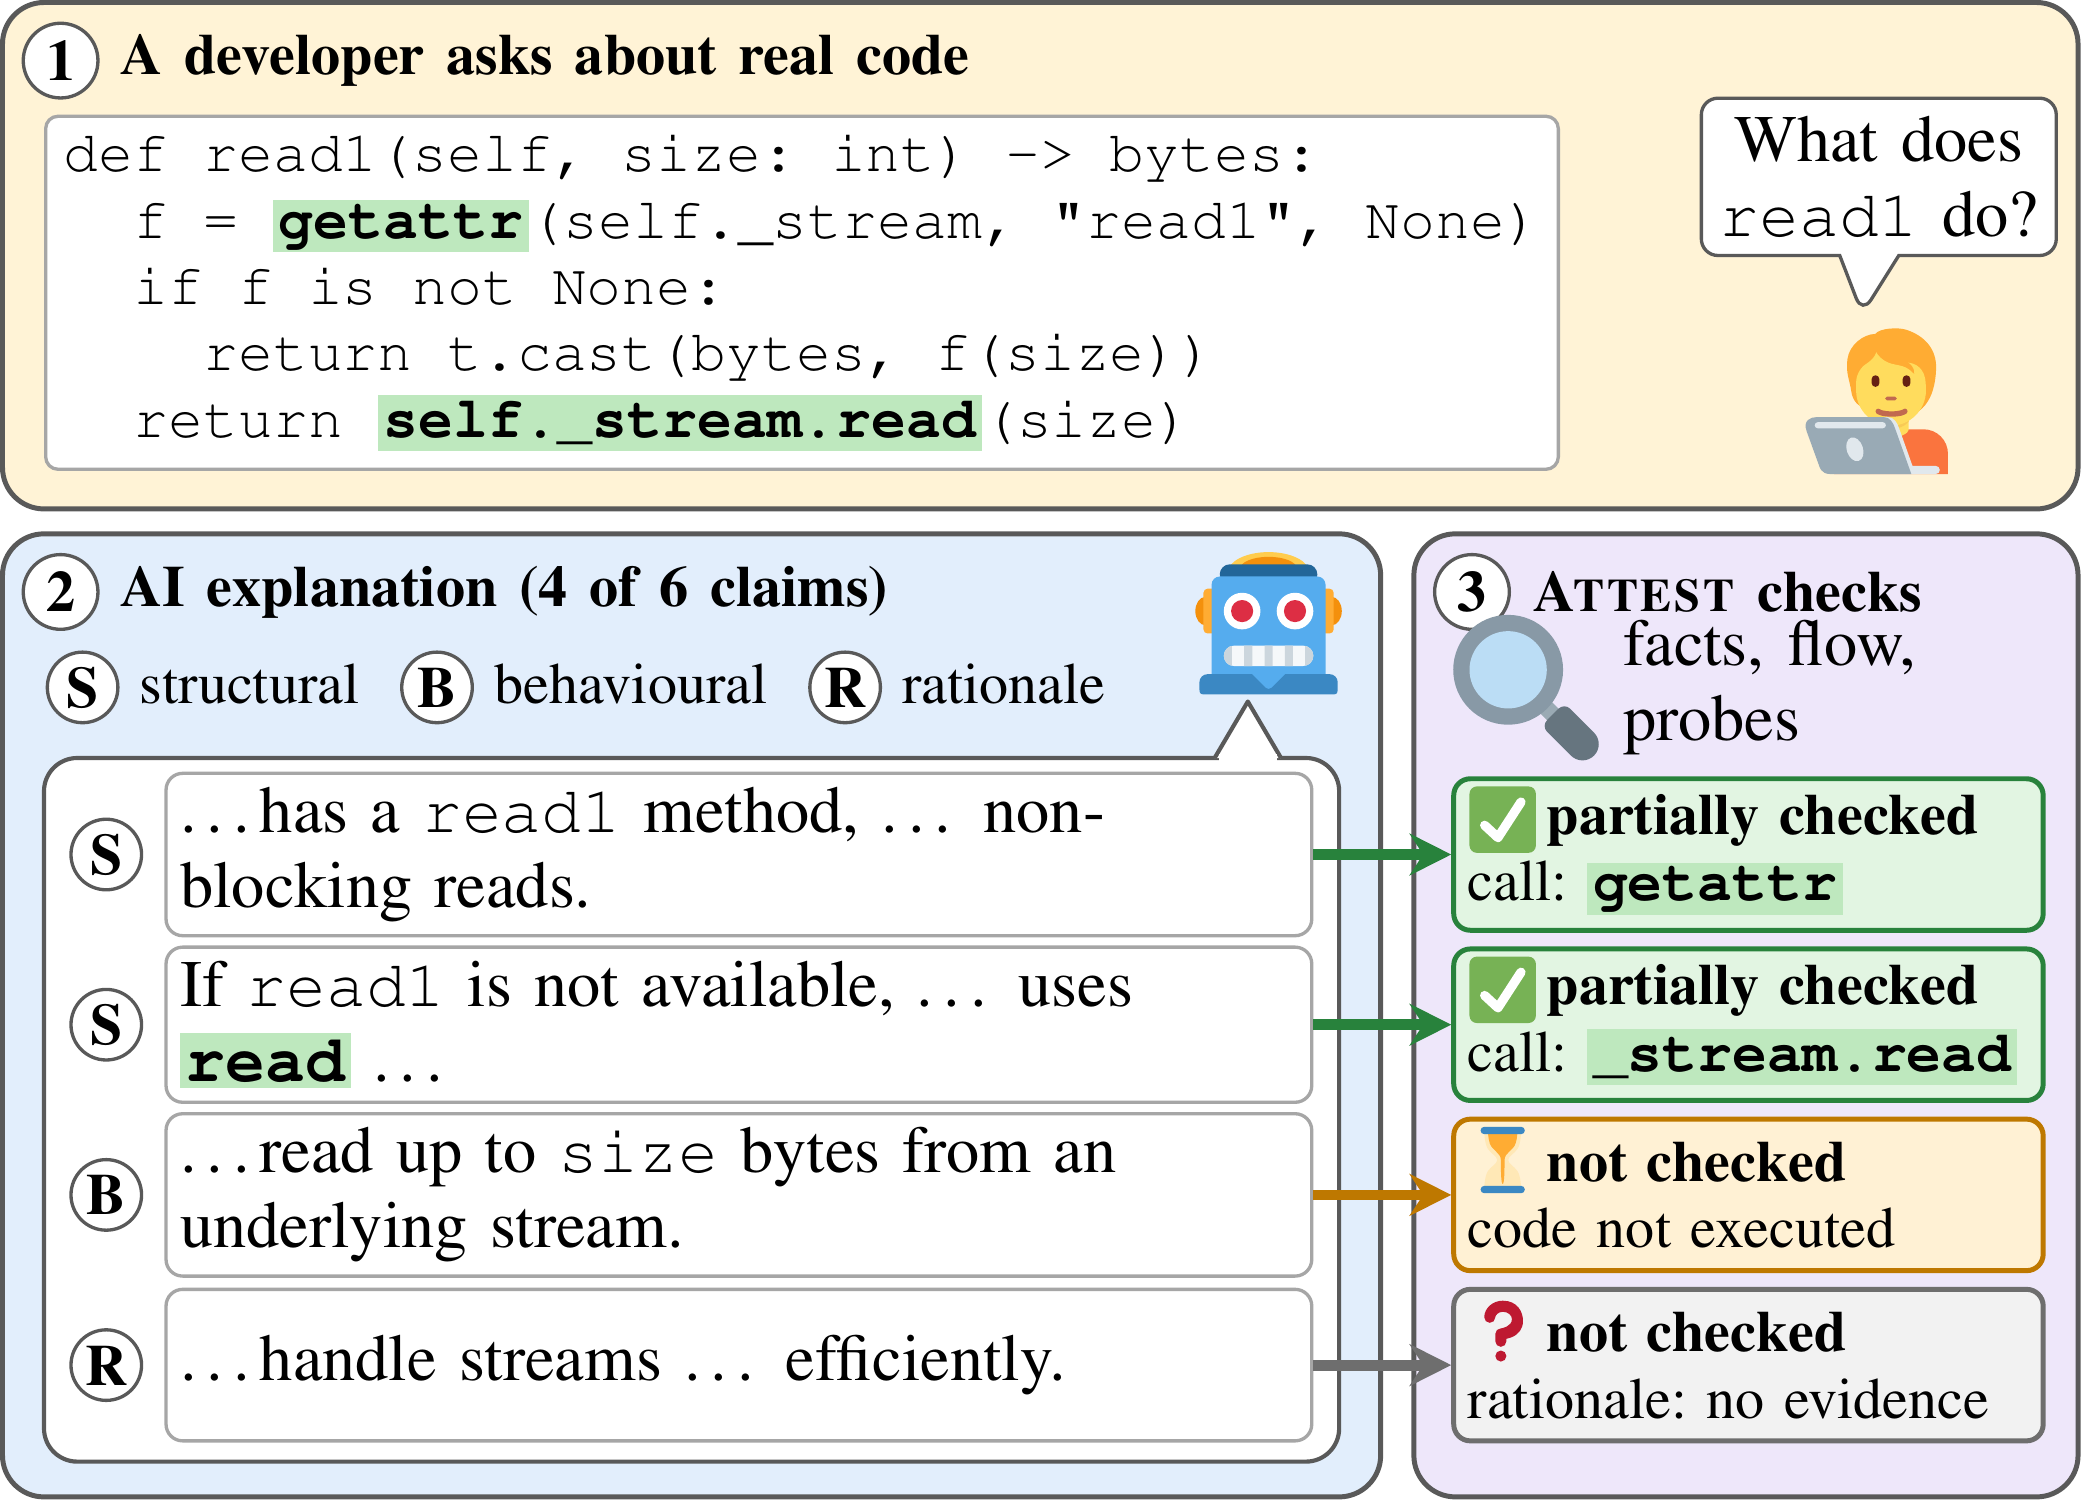
\includegraphics[width=249.664bp,height=179.925bp]{figures/figure1.png}\par\nointerlineskip
\caption{Evidence supports a specific proposition within an explanation. Four shortened claims about \texttt{read1} show supported calls alongside unassessed conditions and behaviour.}
\label{fig:example}
\end{figure}

We make that distinction explicit through evidence \emph{kind}, the source available to assess a claim, and \emph{scope}, exactly what that source supports. A \emph{slot} is an extracted field, such as a called function's name, from which we form a checkable proposition. Our \emph{slot-support contract} pairs that proposition with the surrounding content left unassessed. It makes explicit why a call-name match can coexist with an unchecked condition in the same sentence.

This focus complements the work of Sistla et al.~\cite{sistla2025verified}, our closest comparison, who verify explicit logical statements with correctness guarantees. With \attest{}, we examine code occurrences, possible value transfers and input-specific tests under an explicit scope contract. Our contribution connects these evidence kinds to sentence scope through an inspectable contract and paired diagnostics.

In an audit of our reproducible sample of 40 supported targets, an AI assistant tentatively classified 34 as partial or unrelated matches to their sentences. Our retrospective evaluation traces this mismatch through coverage and extraction. We then use simulations to prepare a study testing whether explicit evidence scope improves sentence judgments.
